\section{Modeling}

The proposed model consists of three distinct phases: a convolutional preprocessor, an attention layer (as discussed in Section 3), and a classifier. 

\begin{figure}[H]
\caption{The proposed architecture. Red arrows represent dropout connections.}
\label{fig:mod}
\centering
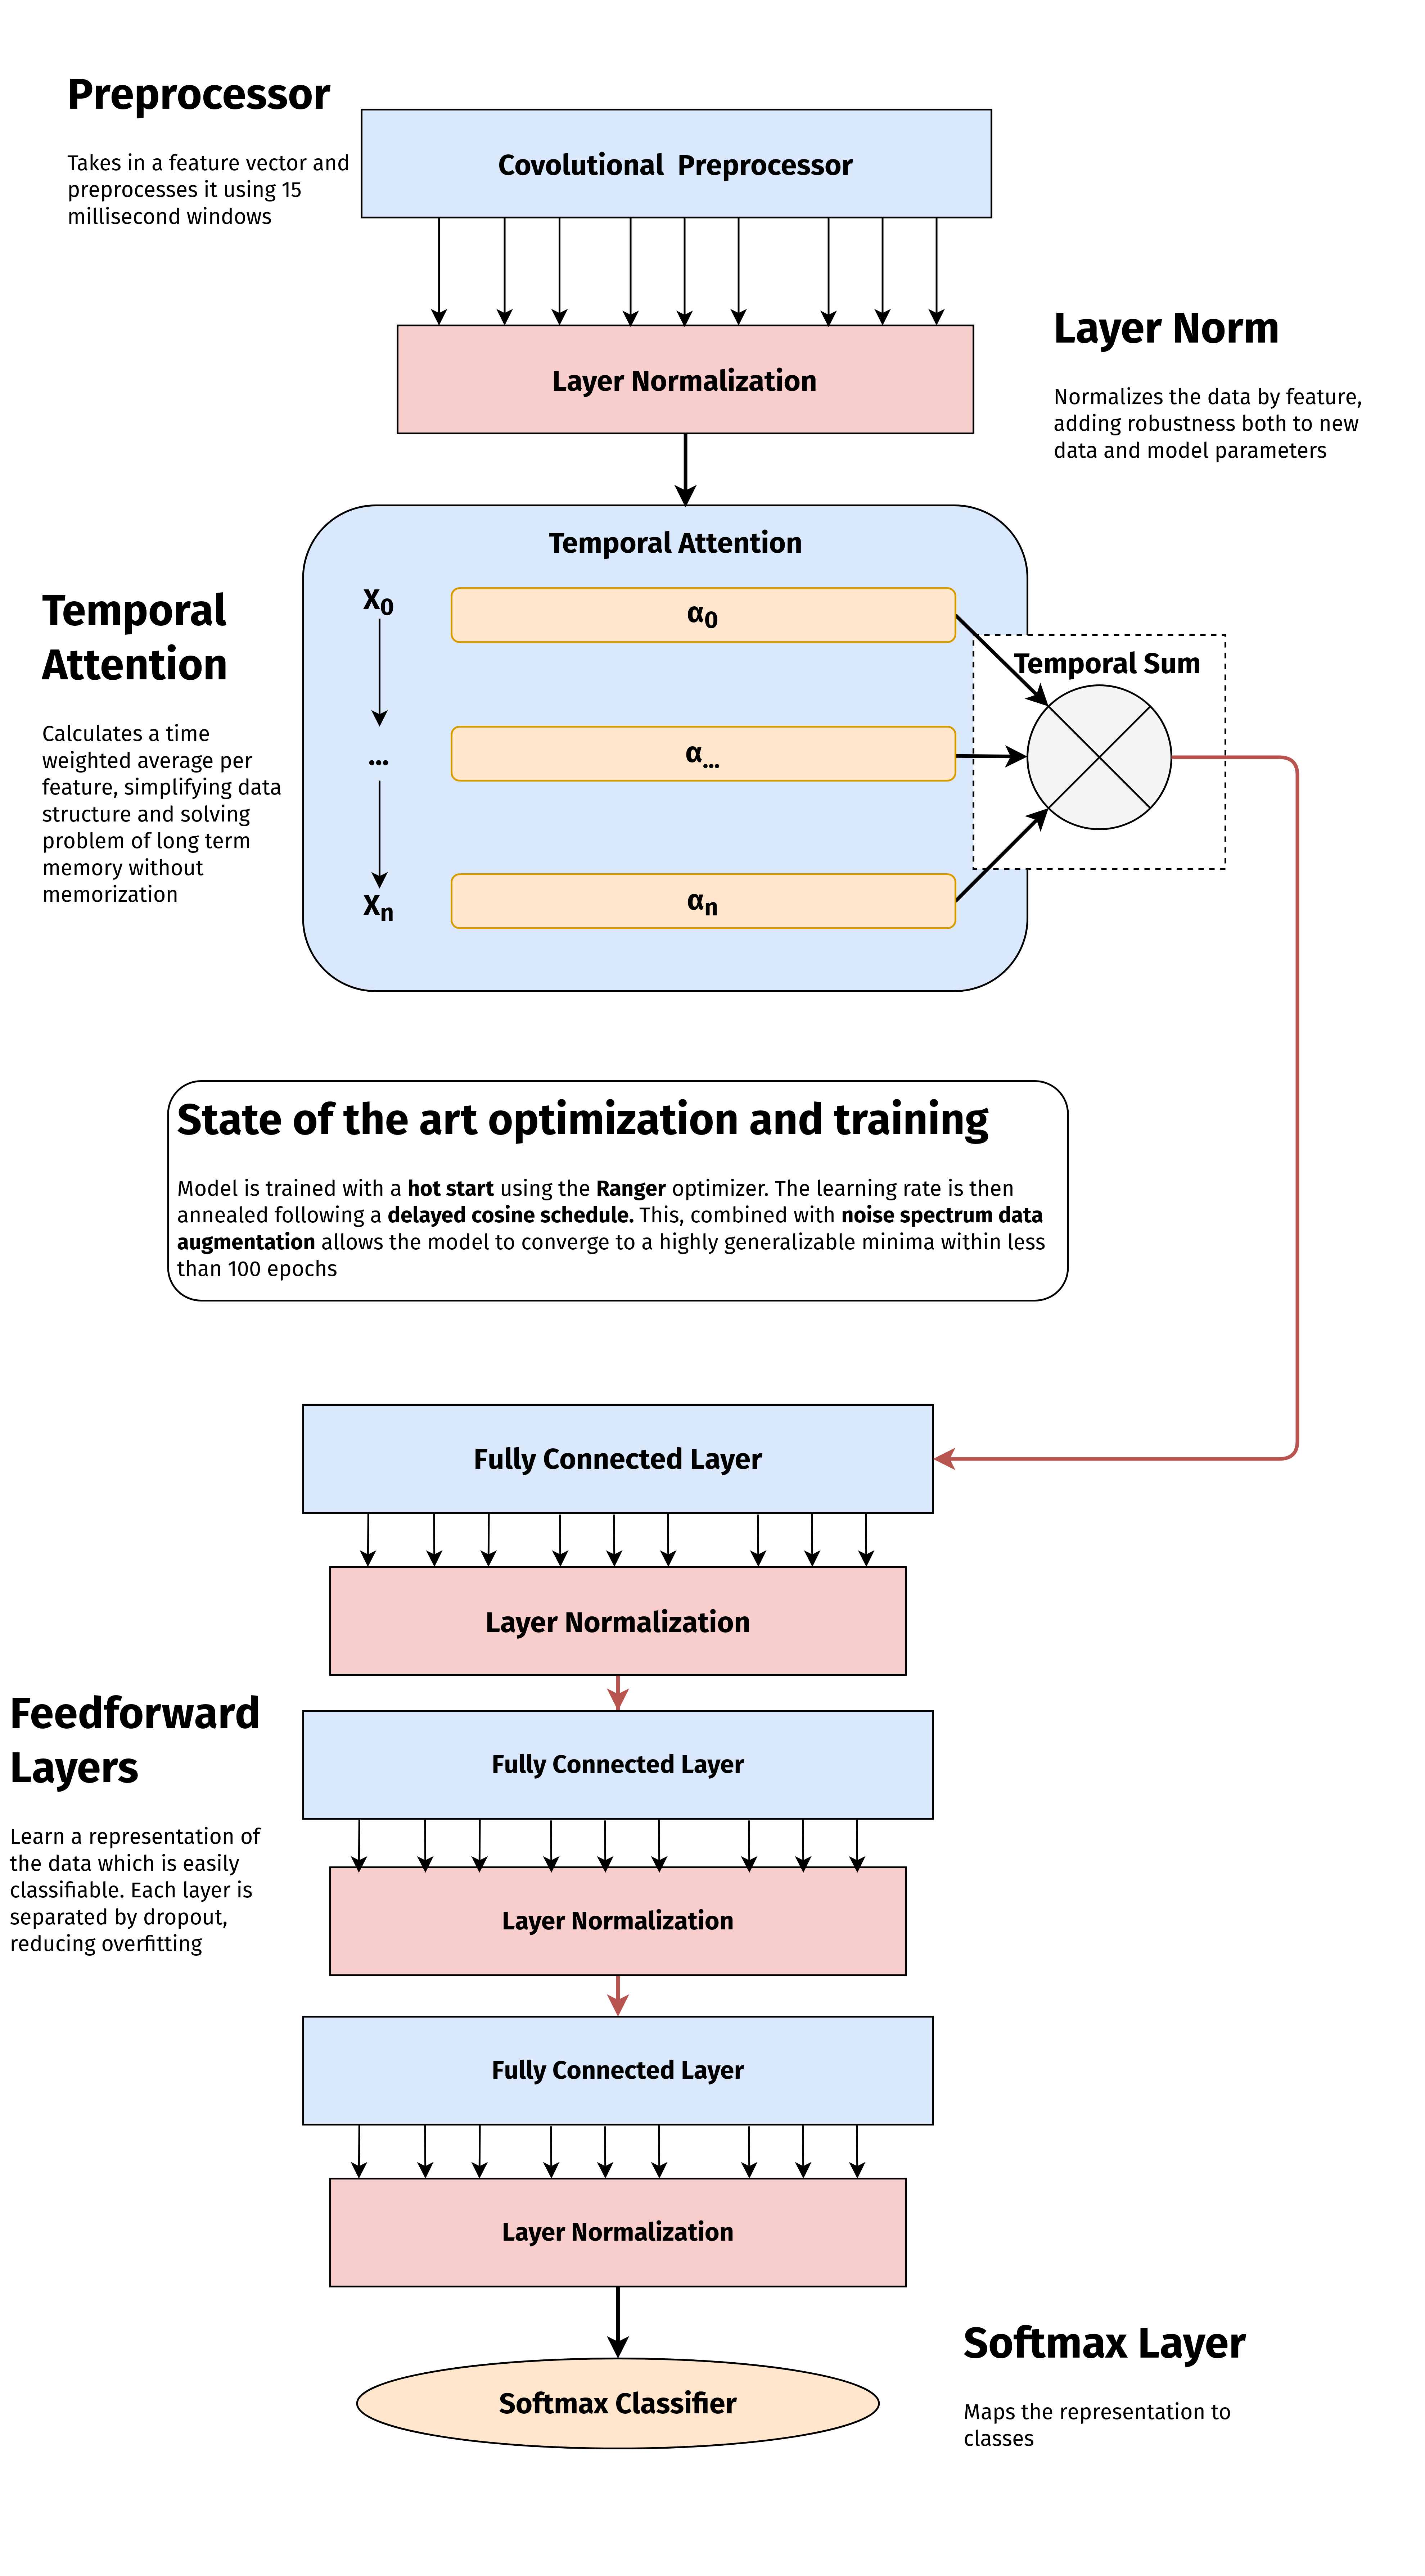
\includegraphics[width=\textwidth]{ntall}
\end{figure}

As seen in \autoref{fig:mod}, the first stage of the model consists of a single, 1-dimensional convolutional preprocessing layer. This  layer takes in the processed time series data, and filters them with a kernel size of three. That is, every three timesteps is filtered down into a single value (for each channel). This is done for each timestep, with 128 filters, resulting in a $(M, 128)$ matrix (where $M$ is the length of the time series). The output of this layer, and the output of all subsequent layers, are normalized across features (layer normalization) \cite{layernorm}. Layer normalization differs from batch normalization in that it normalizes across features, instead of across batches. Mathematically, consider a batch with dimensions $\bm{\left(\mathrm{samples }, \mathrm{timesteps }, \mathrm{features }\right)}$ (or, after attention, $\bm{\left(\mathrm{samples }, \mathrm{features }\right)}$). When batch normalization is applied, the weights are normalized using summary statistics across the \emph{samples}, while with layer normalization, the summary statistics used to normalize the weights are calculated across the \emph{features}.
\par
This matrix is then fed into the feed-forward attention mechanism described in \autoref{fig:okokt}, resulting in a feature vector of 128 values. These are fed into the classification network, which consists of a set of standard, feed-forward layers. The arhitecture of the classifier is based off of the architecture proposed  in \cite{dbn}, and was chosen due to its ability to effectively represent complex data. The output of this network is softmaxed in order to produce the final classifications. Each layer of the classification network is regularized using dropout.

\subsection{Training}

Several state of the art training techniques were employed in this model. First, instead of using the ReLU activation function, all layers use the "Mish" activation function \cite{mish}. The Mish activation function is slightly less regularized then ReLU, thus yielding results slightly faster (and avoiding the "dead neuron" problem). Instead of optimizing the network with Adam or SGD, the model was optimized using the Ranger optimizer. The Ranger optimizer consists of two components: Rectified Adam (RAdam) and Lookahead. The RAdam algorithm represents an improvement over the Adam optimizer in that it does not require a "warm up period", which Adam is notorious for needing. This allows the model to be trained to an optima much faster \cite{radam}. The Lookahead algorithm works in conjunction with a primary optimizer. The primary optimizer calculates weights as it normally does, and then the lookahead optimizer explores the loss landscape near the calculated weights. This allows for even faster convergence to an optima \cite{ranger2}. The combination of Lookahead and RAdam is the Ranger optimizer used in this paper \cite{ranger1}. Due to the very hot start of this combination (Mish and Ranger), the model learns very quickly. To further speed up training, the learning rate followed a delayed cosine annealing schedule. For the first 5 epochs, the model trains at a very high learning rate, and is subsequently annealed over the course of 50 epochs to a very low learning rate. This allows the model to quickly propel itself to a flat optima, and then work towards the bottom. This "hot start" methodology allows the model to quickly converge to a robust local minima \cite{break}.

A significant issue in sEMG classification is the large class imbalance present in the data. Most of the time, the hand is at rest. In the Nina 5 dataset, this means that there was over 30 times rest as any of the other 53 classes (and this also means that a non movable prosthetic hand would be about 60\% accurate). Three methods were tested to combat this imbalance. First, undersampling the majority class (rest), so that it would have the same likelihood of occurring in the training dataset as the other classes yielded decent results. A similar approach, augmenting all the minority classes to match the majority class, was tested, however the slight benefit over undersampling was far outweighed by the prohibitive training cost of this method. Finally, a loss-based method was tested, using focal loss \cite{focal}. Focal loss is calculated in almost exactly the same manner as categorical cross entropy, except it gives a lower importance to well aligned (easy to classify) samples, and raises the importance of difficult samples. This yielded by far the best results. 
